\documentclass{article}
\usepackage[utf8]{inputenc}
\usepackage[russian]{babel}
%\usepackage{systeme}
\usepackage{amsmath}
\usepackage{amssymb}
\usepackage{amsfonts}
\usepackage{mathtext}


%\usepackage[dvips]{graphicx}
\usepackage[final]{graphicx}
\graphicspath{{noiseimages/}}

\renewcommand{\baselinestretch}{1.5}

\title{Пятое задание по БМСО}
\author{Ярослав Аверьянов}
\date{Ноябрь 2015}

\begin{document}

\maketitle

Пусть задана выборка $D = (X, \mathbf{y}) = {(\mathbf{x_i}, y_i = y(\mathbf{\mathbf{x_i}}))}_{i=1}^n$ - выборка из $n$ значений функции $y(\mathbf{x_i})$ в точках $\mathbf{x_i}, i = 1,...,n$. Задана ковариационная функция гауссовского процесса $k_{\mathbf{\theta}}(\mathbf{x},\mathbf{x^{'}})$ из параметрического семейства ${k_{\mathbf{\theta}}(\mathbf{x}, \mathbf{x^{'}}), \mathbf{\theta} \in \Theta}$.

\section{Первая задача}
\begin{center}
$p(\mathbf{x}) = N(\mathbf{x}|\mathbf{\mu}, \Lambda^{-1}),$\\
$p(\mathbf{y}|\mathbf{x}) = N(\mathbf{y}|A\mathbf{x} + \mathbf{b}, L^{-1})$
\end{center}
Покажем, что:
\begin{center}
$p(\mathbf{y}) = N(\mathbf{y}|A\mu + \mathbf{b}, L^{-1} + A\Lambda^{-1}A^{T}),$\\
$p(\mathbf{x}|\mathbf{y}) = N(\mathbf{x}|\Sigma A^{T}L(\mathbf{y} - \mathbf{b}) + \Lambda\mu,\Sigma),$\\
где $\Sigma = (\Lambda + A^{T}LA)^{-1}.$
\end{center}
У нас $p(x) \sim exp(-\frac{(x - \mu)^{T}\Lambda(x - \mu)}{2})$\\
$p(y|x) \sim exp(-\frac{(y - Ax -b)^{T}L(y - Ax - b)}{2})$\\
Здесь $x \sim N(\mu, \Lambda^{-1})$ и $\epsilon \sim N(0,L^{-1})$.\\
Далее возьмем следующую СВ: $y^{'} = Ax + b + \epsilon$ и для нее выполняется равенство: $p(y^{'}|x) = p(y|x) \to y^{'} \sim y;$\\
$Ax + b \sim N(A\mu + b, A\Lambda^{-1}A^{T}).$\\
$Ax + b + \epsilon$ - также гауссовский процесс с математическим ожиданием $A\mu + b$ и с корреляционной матрицей:\\
$\mathbf{E}[(Ax - A\mu + \epsilon)(Ax - A\mu + \epsilon)^{T}] = \mathbf{E}[(Ax - A\mu)(Ax - A\mu)^{T}] + 2\cdot E[(Ax - A\mu)\epsilon^{T}] + \mathbf{E}[\epsilon\epsilon^{T}] = \mathbf{E}[(Ax - A\mu)(Ax - A\mu)^{T}] + \mathbf{E}[\epsilon\epsilon^{T}] = A\Lambda^{-1}A^{T} + L^{-1} \to y \sim N(A\mu + b, A\Lambda^{-1}A^{T} + L^{-1});$\\
Т.к. $y = Ax + b + \epsilon \to \epsilon = y - b - Ax$. Для данной точки $(x,\epsilon)$ плотность в ней $\sim exp(-\frac{(x-\mu)^{T}\Lambda(x-\mu)}{2})\cdot exp(-\frac{(y-Ax-b)^{T}L(y-Ax-b)}{2}) \sim exp(-\frac{x^{T}(\Lambda + A^{T}LA)x - 2x^{T}(\Lambda\mu + A^{T}(y-b))}{2}).$\\
$\to p(x|y) \sim N(\Sigma(\Lambda\mu + A^{T}(y - b)), \Sigma),$ где $\Sigma = (\Lambda + A^{T}LA)^{-1}$.   


\section{Вторая задача}
Покажем, что для $\theta < 0$ функция $k_{\theta}(x,x^{'}) = exp(-\theta(x - x^{'})^2)$ не может быть ковариационной функцией гауссовского процесса для $x \in \mathbf{R}$\\
Мы имеем, что $-\theta(x - x^{'})^2 \geq 0 \to exp(-\theta(x - x^{'})^2) \geq 1 \to k_{\theta}(x, x^{'}) \geq 1$\\
Далее воспользуемся неравенством Коши-Буняковского:\\
$k(X(t_1), X(t_2)) = \mathbf{E}[X(t_1),X(t_2)] \leq \sqrt{\mathbf{E}[X^2(t_1)]} \cdot \sqrt{\mathbf{E}[X^2(t_2)]} = 1$\\
$\to$ Противоречие.

\section{Третья задача}
LR:
\begin{center}
$y(t) = \sum\limits_{q=1}^{Q} x_q(t)\beta_{q} + \epsilon(t)$\\
При $t = t_{i} \forall i = 1,...,n$\\
$\epsilon(t_i) \sim N(0,\sigma_{\epsilon}^2)$ и $\beta_q \sim N(0,a_q)$\\
\end{center}
$\to cov(y(t_i), y(t_j)) = \sum\limits_{q=1}^{Q} a_q x_q(t_i)x_q(t_j) + \delta_{ij}\sigma_{\epsilon}^2$\\
$\to LR $ может быть переписана как GPR:
\begin{center}
$y(t) = f(\vec{x}(t)) + \epsilon(t)$ или $y(\vec{x}) = f(\vec{x}) + \epsilon(\vec{x})$\\
где $\vec{x} = (x_1,...,x_{Q}),\quad f(\cdot) \sim GP(0,k_{linear}(\cdot,\cdot)),$\\
$k_{linear} = \sum\limits_{q=1}^{Q}a_q x_q x_q^{'}$
\end{center}

\section{Четвертая задача}
$D_{-j} = [(\mathbf{x_i}, y_i = y(\mathbf{x_i}))]_{i = 1,...,j-1,j+1,...,n}$.\\
$\hat{y_{-j}} = \mathbf{E}[p(y(\mathbf{x_j})|D_{-j}, \mathbf{\theta})]$ в точке $\mathbf{x_j}$ с ковариационной матрицей $k_{\theta}(\mathbf{x}, \mathbf{x^{'}})$ и выборкой $D_{-j}$.
\begin{center}
Получить выражение для $\sum\limits_{j=1}^{n} (\hat{y_{-j}} - y_j)^2$.
\end{center}
Обозначим $K_{ij} = k_{\theta}(x_i, x_j)$ и введем диагональную матрицу $R_{\theta}$, на диагонали которой находятся диагональные элементы $K^{-1}$.\\
Тогда мы пытаемся найти $\hat{\theta} : \hat{\theta} \in argmin \sum\limits_{i=1}^{n} (y_i - \hat{y_{\theta, -i}})^2$.\\
Тогда если поочередно рассматриваить каждый элемент суммы, то минимум достигается при:\\
$\hat{y}_{-i} - y_{i} = \frac{e_i^{T}K^{-1}y}{e_i^{T}K^{-1}e_i}$, где $e_i$ - $i$ый единичный орт.\\
Т.е. $y_i - \hat{y}_{\theta,-i} = \frac{1}{(K^{-1})_{i,i}}(K^{-1}y)_{i}$. Тогда $\sum\limits_{i=1}^{n} (y_i - \hat{y}_{\theta,-i})^2 = y^{T}K^{-1}R_{\theta}^{-1}R_{\theta}^{-1}K^{-1}y$.



\section{Пятая задача}
В этой задаче нужно было сравнить работу 4 алгоритмов добавления точки на $n$-ом шаге:\\
1.Новая точка добавляется случайно.\\
2.Новая точка максимизирует минимальное расстояние до точек текущей выборки $D_n$.\\
3.Новая точка максимизирует апостериорную дисперсию гауссовского процесса для $D_n$.\\
4.Новая точка минимизирует ошибку аппроксимации на заданной тестовой выборке $D_{test}$, если добавить ее к текущей выборке $D_n$.\\
Мною использовалась функция $f(x, y) = -(x^2 + y^2)$.\\

\begin{figure}[h]
\center{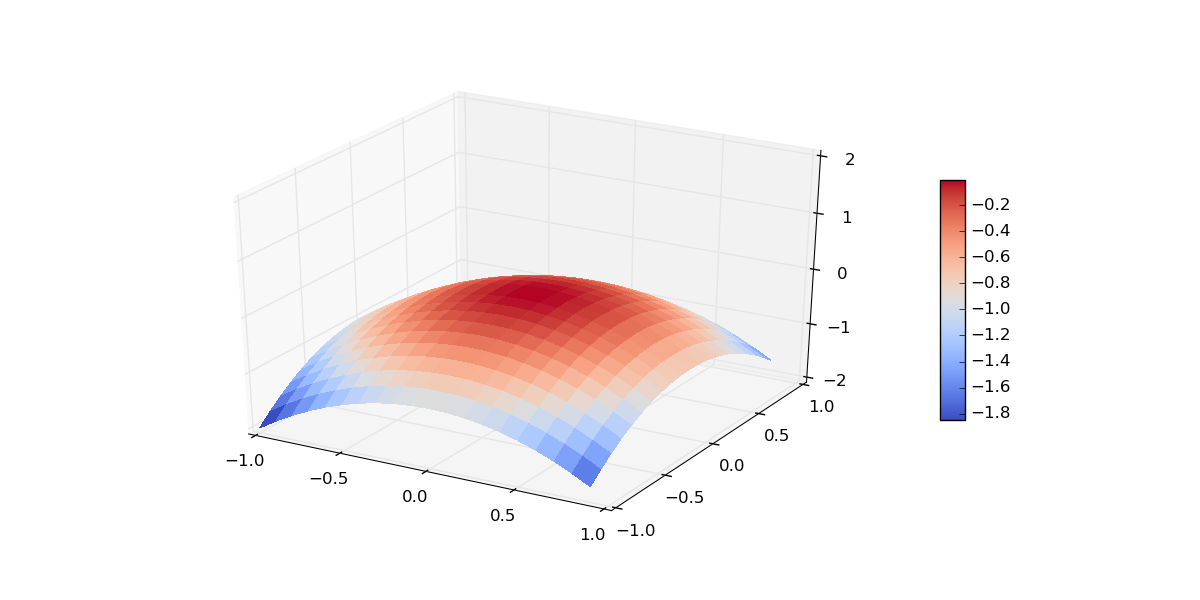
\includegraphics[width=1\linewidth]{figure_1}}
\caption{$f(x,y) = -(x^2 + y^2)$}
\label{ris:image}
\end{figure}

Начальный дизайн - выборка размера 30 из $\mathbf{U}([0,1]^2)$.\\
Точки-кандидаты - выборка размером 30 из $\mathbf{U}([0,1]^2)$.\\
Тестовая выборка - выборка размером 40 из $\mathbf{U}([0,1]^2)$.\\
В результате был построен график среднеквадратичной ошибки на тестовой выборке после добавления
новой точки. Лучший алгоритм - четвертый алгоритм, худший - первый алгоритм .\\
\begin{figure}[h]
\center{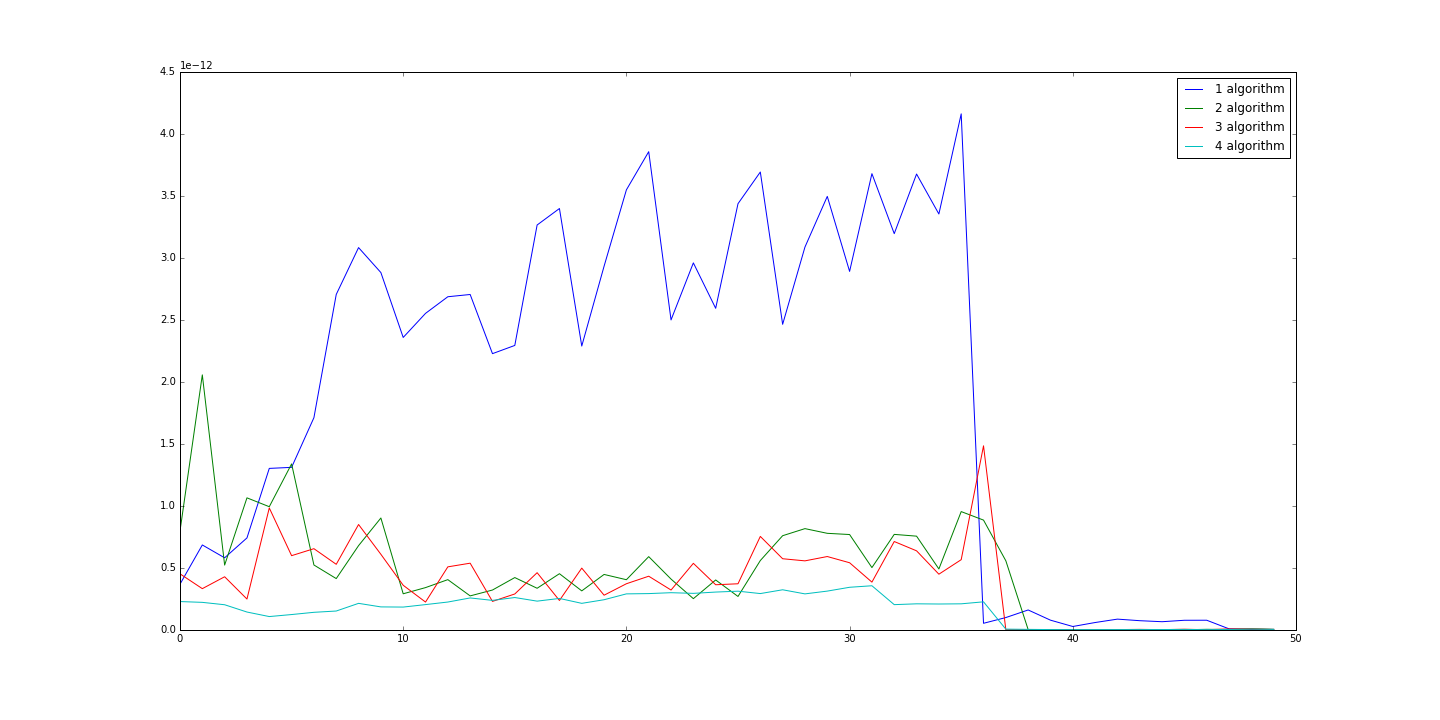
\includegraphics[width=1\linewidth]{figure_2}}
\caption{Среденеквадратичная ошибка на тестовой выборке в зависимости от количества точек, добавляемых в обучаемую выборку}
\label{ris:image}
\end{figure}

\end{document}

